\documentclass[11pt,a4paper]{globis-book}

\usepackage{graphicx}
\usepackage[helvetica]{quotchap}
\usepackage{times}
\usepackage{ethfont}
\usepackage[british]{babel}
\usepackage{longtable}
\usepackage{fancyhdr}
\usepackage{shadethm}
\usepackage{makeidx}
\usepackage[a4paper,portrait,twoside,inner=3.25cm,outer=3.5cm,top=3.5cm,bottom=4.0cm]{geometry}
\usepackage{hyperref}
\usepackage{globis}

\renewcommand{\sectfont}{\sffamily\bfseries\Huge}

\setlength{\shadedtextwidth}{\textwidth}
\setlength{\shadeleftshift}{3mm}
\setlength{\shaderightshift}{3mm}
\addtolength{\shadedtextwidth}{-\shadeleftshift}
\addtolength{\shadedtextwidth}{-\shaderightshift}
\setlength{\parindent}{0pt}
\setlength{\parskip}{5pt}

\sloppy

\pagestyle{fancy}
\fancyhf{}
\fancyhead[LE,RO]{\sffamily\bfseries\small\thepage}
\fancyhead[LO]{\sffamily\bfseries\small\leftmark}
    \fancyhead[RE]{\sffamily\bfseries\small\rightmark}
\renewcommand{\headrulewidth}{0.1pt}
\renewcommand{\footrulewidth}{0pt}

\fancypagestyle{plain}{
    \fancyhf{}
    \fancyfoot[C]{\sffamily\bfseries\small\thepage}
    \renewcommand{\headrulewidth}{0pt}
    \renewcommand{\footrulewidth}{0pt}
}

% Please adapt the following fields if necessary!
\hypersetup{
    pdftitle = Distributed Ph Tree, 
    pdfauthor = Bogdan Vancea,
    pdfsubject = Master Thesis,
    hidelinks,
    plainpages = false,
    bookmarksnumbered = true
} 

\raggedbottom

% Please adapt the following fields if necessary!
\title{Cluster-Computing and Parallelisation for the
    Multi-Dimensional PH-Index}
\category{Master Thesis} 
\author{Bogdan Aurel Vancea}
\email{$<$bvancea@student.ethz.ch$>$}
\professor{Prof. Dr. Moira C. Norrie}
\assistant{Tilmann Zaeschke \\Christoph Zimmerli}
\group{Global Information Systems Group}
\institute{Institute of Information Systems}
\department{Department of Computer Science}
\school{ETH Zurich}
\version{}
\date{\today}
\copyrightyear{2014}

\makeindex

\begin{document}

\frontmatter
\maketitlepage
\cleardoublepage
\pdfbookmark{Contents}{toc}

\chapter*{Abstract}

Here comes the abstract.

\tableofcontents

\mainmatter

% Here comes the content

\chapter{Introduction}
\label{ch:intro}
This chapter briefly describes the context and the motivation of the thesis and presents the objectives that are to be achieved. Finally, section \ref{sec:intro-outline} provides an overview of this thesis.

\section{Motivation}
\label{sec:intro-motivation}
Multi-dimensional data is widely used today, especially in domains like database management systems, geographic information systems, computer vision and computational geometry. When all of the dimensions of the data hold numerical values, this data can be viewed as a collection of points in higher dimensional spaces. Due to this nature, multi-dimensional numerical data provides the possibly of posing more complex queries based on the distance between these points in space. For example, in the context of a geo-information system, one could query for all of the points that fall inside a specific hyper-rectangle or attempt to find the nearest neighbours of an arbitrary query point.

Several point-based multi-dimensional indexing solution have been developed in the latest years, the most prominent being kD-trees~\cite{Bentley1975} and quadtrees~\cite{FinkelB74}. This type of data structures store the multi-dimensional data such that more complex operations, like range and nearest neighbour queries are executed efficiently. The PhTree~\cite{Zaschke2014} is a new multi-dimensional data structure based on the quadtree. In addition to providing support for complex queries, the PhTree is also space-efficient, as its space requirements are sometimes even lower than those of multi-dimensional arrays. 

As technology advances and the world becomes more connected, multi-dimensional data becomes easier to acquire and store. Because of this, it is necessary that multi-dimensional data structure need to store and manage more data than would fit a single machine. However, traditional multi-dimensional indexes like the kD-tree and quad-tree do not cover this use case as they are designed to run on a single machine.

Additionally, in the last few years the processor speed has reached the power wall and processor designers cannot increase the CPU frequency by increasing the number of transistors. Recent advances in processor design have been made by adding more cores on CPU's rather than increasing the processing frequency. Therefore, it is important that contemporary data structures be adapted to multi-core architectures by allowing them to support concurrent accesses. As with the case of the increase storage requirements, traditional multi-dimensional data structures do not support concurrent write operations.

This thesis attempts to provide a solution to these two issues by extending the PhTree multi-dimensional index to run on distributed cluster of machines. Furthermore, the PhTree is also updated to support concurrent access.

\section{Objectives}
\label{sec:intro-objectives}
The previous section has highlighted two challenges currently faced by indexing systems: \textit{high storage requirements} and \textit{support for concurrent access.}. This work proposes the distributed PhTree, a version of the PhTree that can be run on a cluster of machines, making it able to handle data sets that cannot fit in the main memory of a single machine. Moreover, the distributed PhTree should be able to handle concurrent requests. This applies both to requests sent to different machines that are part of the cluster and concurrent requests sent by different clients to the same machine. 

Specifically, the distributed PhTree has to fulfill the following requirements:
\begin{description}
    \item[Cluster capability] The system should run across a network of machines, making use of the memory and processing resources on each machine. Furthermore, the system should attempt to balance the number of multi-dimensional entries that each machine is responsible of.
    \item[Cluster concurrency] The system should be able to support concurrent requests to different nodes of the cluster. Each node should be able to process queries related to the entries that it stores locally.
    \item[Node concurrency] Each node should support multi-threaded read and write access to the entries that it stores.
\end{description} 

As the thesis touches on two main subjects, distribution and concurrency, the main challenges encountered are twofold. From the distribution perspective, the challenges are the identification of suitable entry distribution and balancing strategies, devising efficient algorithms for executing queries across multiple cluster nodes, and the efficient management of a very large number of cluster nodes. For the concurrency perspective, the challenges are the identification of a suitable concurrent access strategy that can maximize the number of concurrent write operations.

\section{Thesis outline}
\label{sec:intro-outline}

This chapter gave an overview of the challenges currently faced by multi-dimensional indexing structures and briefly explained how this work seeks to address them. Additionally, this chapter also presented the main objectives of this thesis. The rest of the thesis is structured as follows:

\textbf{Chapter \ref{ch:background}} provides additional information about the PhTree, its characteristics and supported operations. The second part of this chapter describes relevant previous work done in the areas of distributed multi-dimensional indexes and concurrent data structures.

The design of the distributed PhTree from the point of view of a distributed system is presented in \textbf{Chapter \ref{ch:distindex}}. This chapter presents the chosen data distribution strategy, and also touches on the possible alternatives and the consequences of this choice. Additionally, this chapter provides an overview of how the queries spanning multiple nodes are executed by the system.

The addition of the multi-threaded read and write support for the PhTree is discussed in \textbf{Chapter \ref{ch:concurrency}}. Several concurrent access strategies are discussed, together with their advantages, disadvantages and consistency guarantees.

\textbf{Chapter \ref{ch:implementation}} describes the implementation-specific decisions that were taken during the development process. This chapter also presents the technologies that were used and justifies the technological choices.

The distributed PhTree is evaluated in \textbf{Chapter \ref{ch:evaluation}}. The performance characteristics of the implemented distributed systems as well as those of the implemented concurrency strategy are discussed.

\textbf{Chapter \ref{ch:conclusions}} concludes the thesis by presenting the contribution of this work in the context of distributed multi-dimensional indexing systems. This second part of this chapter discusses possible future contributions.

\chapter{Background}
\label{ch:background}
The first part of this chapter analyses the single-threaded PhTree, a multi-dimensional data structure and the starting point of this work. It provides an overview of its specific characteristics and describes the supported operations.

The second part of this chapter presents the relevant related work in the area of distributed multi-dimensional index and concurrent data structures. 

\section{The PhTree}
\label{sec:background-phtree}

The PhTree~\cite{Zaschke2014} is a novel multi-dimensional indexing structure that focuses on fast retrieval and highly efficient storage. It combines concepts from PATRICIA-tries, quadtrees and hypercubes to encode the multi-dimensional data using bit prefix sharing. Because of this, the storage requirements can sometimes be lower than those of the storage requirements of an array of objects.

An example PhTree storing 2-dimensional 4 bit points is shown in \ref{fig:PhTree-example}. The tree illustrated in this figure stores the points: (0, 4), (3, 4) and (3, 6). However, each point is stored as the \textit{bit interleaving} of its values in all dimensions. Therefore, the bit interleaving of point (3, 6), represented in binary as (0011, 1010) is 01001110. By storing the points under the \textit{bit interleaving} form, the PhTree maps the multi-dimensional points into a 1-dimensional space. The 1-dimensional values will be referred to as \textit{Z-values} as they form the \textit{Z-order space filling curve}. 

\begin{figure}[h]
    \centering 
    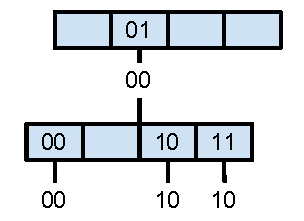
\includegraphics{images/PhTree-example}
    \caption{2 dimensional 4bit PhTree containing the points: (0000, 1000), (0011, 1000), (0011, 1010).}
    \label{fig:PhTree-example}
\end{figure}

The PhTree has the following important properties:
\begin{itemize}
    \item \textbf{Z-Ordering}. The multi-dimensional entries are order according to the Z-order space filling curve. As a consequence, points which are close in the original multi-dimensional space will also be relatively close in the Z-Ordering.
    \item \textbf{Constant height}. The height of the PH-tree is equal the number of bits needed to store each value of the multi-dimensional space. Therefore, when the values in each dimension are represented in 64 bits, as long or doubles, the maximum height of the PhTree is 64. This property is important as \textit{the maximum height of the PhTree is independent of the number of points it stores}.
    \item \textbf{Balancing is not needed}. The PhTree does not perform balancing operation after write operation have occurred. While this fact could lead to un-balanced trees, it is usually not a problem in practice, as the height of tree is limited by a constant factor.
\end{itemize}

The PhTree is similar to a HashMap, as it stores entries consisting of key-value pairs. In this case however, the key is a multi-dimensional data point, while the value can be an arbitrary object. The following operations are supported:
\begin{itemize}
    \item \textbf{Point queries} operate on single multi-dimensional points. The possible queries are \textit{get()}, \textit{put()}, \textit{delete()} and \textit{updateKey()}. The \textit{get()} query retrieves the value associated with a multi-dimensional key, and the \textit{delete()} operation removes the value associated with a multi-dimensional key. The \textit{put()} operation adds new key-value to the index. Finally, the \textit{updateKey()} operations updates the key associated with an existing key-value entry.
    \item \textbf{Range queries} select all of the data points that fall inside a multi-dimensional hyper-rectangle. This rectangle is defined by a \textit{lower left} and a \textit{upper right} point. 
    \item \textbf{Nearest neighbour queries} select the closest k points in the index to an arbitrary query point. 
\end{itemize}

\section{Related work}
\label{sec:background-rw}

\textit{Meta - will be removed after editing.}
\textit{Present the relevant related work.}

\subsection{Distributed Indexes}

Distributed Hash Tables (DHT's) are a class of decentralized distributed systems which expose an API similar to that of a hash-table. These P2P systems use a structured overlay network to assign a given key to a node in the system. Requests for a certain key can be sent to any node of the system and will be forwarded to the node responsible for it. DHT's have been designed to work on internet-scale, connecting large numbers of machines across large distances. The main concerns are scalability and availability, while the \textit{get()} and \textit{put()} operations have "best effort" semantics. Chord~\cite{Stoica2001chord}, one of the most popular and most efficient DHT system, manages to guarantee that any request for a certain key will arrive the responsible node in at most \textit{O(logn)} hops, in the context in which each nod contains only \textit{O(logn)} links to other nodes. 

One important issues of distributed hash tables is that they only support "exact match" queries. The Prefix Hash Tree~\cite{Ramabhadran04prefixhash} adds support for range queries to a DHT by using a secondary data structure, to maintain a mapping between nodes and keys. This mapping is a trie containing the prefixes of the bit-strings of the keys, and thus, logically, leaf nodes of this trie correspond to interval regions of keys. All leaf-nods are linked using a linked-list, allowing range queries to traverse the query range starting for the first leaf that matches the range. 

A similar approach is taken by the SkipIndex~\cite{Zhang04skipindex}, a multi-dimensional indexing system that uses a SkipGraph to map geometrical regions to machine nodes. Each system node maintains only a partial view of the region tree and thus range and nearest neighbour queries are performed using selective multicasting.

A different approach for creating a scalable multi-dimensional index is to use a big-data platform. \cite{Liao2010HadoopIndex} propose storing a block-based multi-dimensional index structure like the R-tree directly in HDFS and use query models like MapReduce as building blocks for the implementation of range and nearest neighbour queries.

\subsection{Concurrent data structures}

Concurrent data structures are a highly studied problem in current times. Currently, there are two main ways of implementing a concurrent data structures: lock-based solution and lock-free solutions. Lock-based solutions use locks to synchronize the concurrent access to the either the data structure itself, an approach called \textit{course-grained locking}, or to parts of the data structure, in the approach called \textit{fine grained locking}. Lock-free solutions use either atomic primitives, like \textit{compare-and-swap} or software transactional memory to synchronize modification attempts on the data structure.

In the area of concurrent search trees, lock-based approaches are much more common than lock-free solutions. Fraser ~\cite{Fraser2007concurrent} provides a set of API's that can be used to design arbitrary concurrent data structures. While these API's can be used to for any type of data structures, they are based on software transactional memory or multi-word CAS operations, currently not implemented by contemporary hardware. Brown ~\cite{Brown2014concurrent} presents a general technique for non-blocking trees implemented using multi-word equivalents of the \textit{load-link}(LL), \texit{store-conditional} (SC) and \texit{validate}(VL) atomic primitives.

A naive concurrent implementation of a search tree can be achieved by protecting all access using a single lock. Concurrency can be improved by synchronizing the access at the level of nodes. \textit{Hand-over-hand locking}, something also called \textit{lock-coupling}, is a fine-grained technique that states that a thread can only acquire the lock of a node if it holds the lock of the node's parent node. This technique allows multiple concurrent write operations, but the degree of concurrency is limited due to the fact that all subtrees of a locked node are not accessible, even if the other threads need to perform modifications in a different part of the tree. Another approach is to perform optimistic retries by only locking the nodes that should be modified, check if locked nodes have not been removed from the tree and then perform the update. This idea is used by ~\cite{Bronson2010concurrent} to implement a highly concurrent AVL tree. 

\chapter{Index distribution}
\label{ch:distindex}

\textit{Meta - will be removed after editing.}
\textit{This chapter should focus on how the distributed index was implemented: how the data was split across the cluster nodes, the manner in which the queries are executed and how the entry load balancing is performed.} 

\section{Challenges}
\label{sec:distindex-challenges}

\textit{Meta - will be removed after editing.}
\textit{Present the callenges of implementing a distributed system : scalability, load balancing, etc. Should not focus on issues like security, availability as those are not relevant to this report.}

\section{Distribution strategies}
\label{sec:distindex-strategies}

\textit{Meta - will be removed after editing.}
\textit{Present the possible ways in which the entries can be distributed across the cluster nodes. Talk about the advantages and disaadvantages of each approach. Say which approach was chosen and why.}

\subsection{Hashing}

\subsection{Spatial splitting}

\subsection{Z-Order curve splitting}

\section{Algorithms}
\label{sec:distindex-algorithms}

\textit{Meta - will be removed after editing.}
\textit{This section should explain how the queries should be executed on the distributed system. Present the load balancing algorithm}.

\subsection{Point queries}

\subsection{Range queries}

\subsection{Nearest neighbour queries}

\subsection{Entry load balancing}

\section{Architecture}
\label{sec:distindex-architectures}

\textit{Meta - will be removed after editing.}
\textit{This section should explain how the queries should be executed on the distributed system. Present the load balancing algorithm}.

\chapter{Concurrency}
\label{ch:concurrency}

\textit{Meta - will be removed after editing.}
\textit{Present the concurrency strategies that could be added to the PhTree and explain the consistency model associated with each strategy.}

The PhTree does not currently support concurrent write operations. There are several strategies that could be employed to add concurrent writes.

\section{Challenges}

\section{Concurrency strategies}

\subsection{Copy-on-Write}

\subsection{Locking}

\chapter{Implementation}
\label{ch:implementation}

\textit{Meta - will be removed after editing.}
\textit{Present the implementation architecture and the techologies used.}

\section{System description}
\textit{Meta - will be removed after editing.}
\textit{Describe the system, include class/deployment diagrams.}

\section{Technologies}
\textit{Meta - will be removed after editing.}
\textit{Describe the technologies used, the reasons for which these technologies were chosen and any alternatives.}

\chapter{Evaluation}
\label{ch:evaluation}

\textit{Meta - will be removed after editing.}
\textit{Explain how the system should be evaluated, present and explain the benchmarks}

\chapter{Conclusions}
\label{ch:conclusions}

\section{Contributions}
\label{sec:conclusions-contribution}
\textit{Meta - will be removed after editing.}
\textit{Conclude the report. This should reiterate the main points of the report and try to mirror the introduction}

\section{Future work}
\label{sec:conclusions-future-work}
\textit{Meta - will be removed after editing.}
\textit{Present the points that were not tackled by the thesis and talk about possible future work.}

\appendix

\listoffigures
\listoftables

\chapter*{Acknowledgements}

\newpage
\thispagestyle{empty}

\bibliographystyle{plain}
\bibliography{bibliography}

\end{document} 
